\documentclass{beamer}

\usetheme[hideothersubsections]{Berkeley}
\usecolortheme{seahorse}
\setbeamertemplate{footline}[page number]

\usepackage[utf8x]{inputenc}
\usepackage{amsthm}
\usepackage{amsmath}
\usepackage{alltt}
\usepackage{color}

\author{Filip Jareš, Lenka Mudrová}
\title{Standardní úloha Komár}
\institute{České Vysoké Učení Technické v Praze\\ Fakulta Elektrotechnická}
\date{17.5.2011}

\begin{document}

\begin{frame}
        \titlepage
        \begin{center}
         \begin{figure}[!h]
	\centering
	
\includegraphics[width=0.2\columnwidth]{pics/mosquito}
	%\caption{\cite{komar}}\label{fig:m}
\end{figure}
        \end{center}

\end{frame}

%\pagestyle{plain}
\section{Úvod}
\begin{frame}
\frametitle{Úvod}
 \framesubtitle{}
\begin{enumerate}
 \item Rozbor
 \item Naše řešení
 \item Experimenty
 \item Závěr
\end{enumerate}

\end{frame}

\section{Naše řešení}
\begin{frame}
\frametitle{Hlavní struktura programu}
 \framesubtitle{}
 \begin{itemize}
  \item Spuštění hlavní funkce
  \begin{itemize}
   \item Inicializace serv a kamery
   \item Odvození periody programu přímo od periody získávání obrázků
   \item U videoobjektu zaregistrována callback funkce
   \item Použití každého druhého obrázku
  \end{itemize}

 \end{itemize}
\end{frame}

\begin{frame}
\frametitle{Regulační smyčka}
 \framesubtitle{}
   \begin{itemize}
  \item Vyčtení obrázku, použití pouze zelené složky
  \item Prahování 
  \item Funkce Image Processing Toolboxu
 \end{itemize}
  \begin{figure}[!htb]
	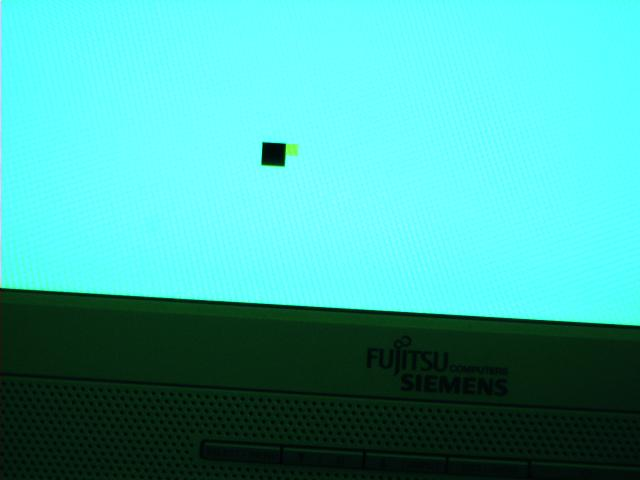
\includegraphics[width=0.49\columnwidth]{pics/zpracovani_obrazu-1}
  \end{figure}
\end{frame}

\begin{frame}
\frametitle{Regulační smyčka}
 \framesubtitle{}
  \begin{itemize}
  \item Vyčtení obrázku, použití pouze zelené složky
  \item Prahování 
  \item Funkce Image Processing Toolboxu
 \end{itemize}
  \begin{figure}[!htb]
	
\includegraphics[width=0.49\columnwidth]{pics/zpracovani_obrazu-2}
  \end{figure}
\end{frame}


\begin{frame}
\frametitle{Regulační smyčka}
 \framesubtitle{}
  \begin{itemize}
  \item Vyčtení obrázku, použití pouze zelené složky
  \item Prahování 
  \item Funkce Image Processing Toolboxu
 \end{itemize}
  \begin{figure}[!htb]
	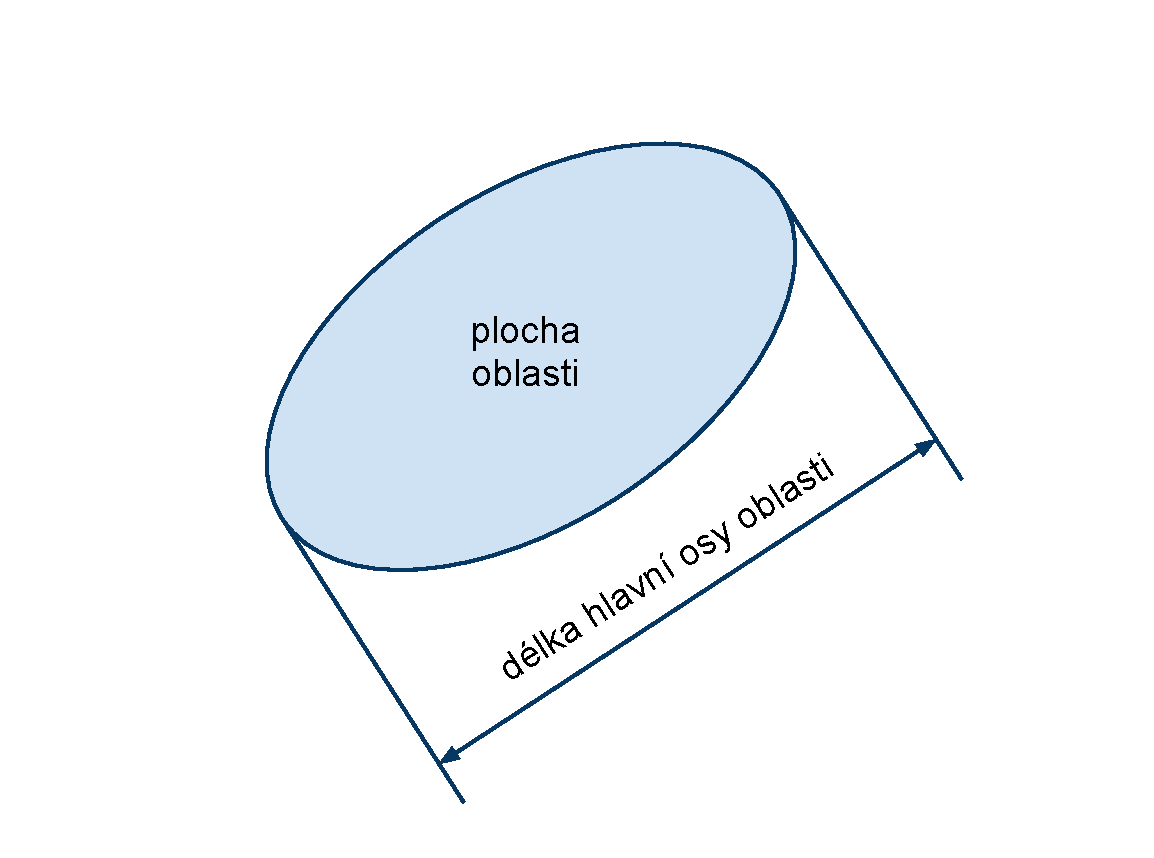
\includegraphics[width=0.49\columnwidth]{pics/delka_hlavni_osy_a_plocha_oblasti}
  \end{figure}
\end{frame}

\begin{frame}
\frametitle{Regulační smyčka}
 \framesubtitle{}
  \begin{itemize}
  \item Vyčtení obrázku, použití pouze zelené složky
  \item Prahování 
  \item Funkce Image Processing Toolboxu
 \end{itemize}
  \begin{figure}[!htb]
	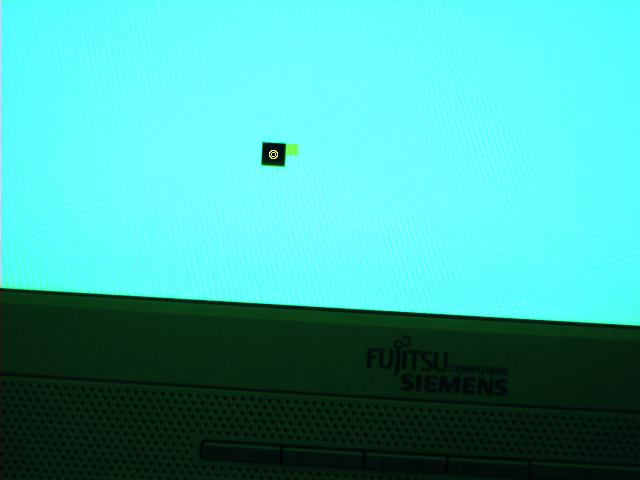
\includegraphics[width=0.49\columnwidth]{pics/zpracovani_obrazu-3}
  \end{figure}
\end{frame}

\section{Experimenty}
\begin{frame}
\frametitle{Experimenty}
 \framesubtitle{}
  \begin{itemize}
   \item Spolehlivá detekce komára
   \item Při accel=300 v průměru sledován 70 s
    
  \end{itemize}

\end{frame}
    
\end{document}
